\documentclass[conference]{IEEEtran}
\usepackage{amsmath}
\usepackage{newtxtext,newtxmath}
\usepackage{graphicx}
\usepackage{booktabs}
\usepackage{tabularx}
\usepackage{array}
\usepackage{seqsplit}
\usepackage{fvextra}
\usepackage{url}
\usepackage[hidelinks]{hyperref}
\usepackage{microtype}
\setlength{\emergencystretch}{2em}
\DefineVerbatimEnvironment{Highlighting}{Verbatim}{breaklines,breakanywhere,fontsize=\small}
\newenvironment{Shaded}{}{}
\title{Does an Exact FIR Sharing Advantage Survive a Stronger Direct Baseline? A Cortex-M0 Model Case Study}
\author{\IEEEauthorblockN{Anonymous authors}}
\begin{document}
\pagestyle{plain}
\maketitle
\thispagestyle{plain}
\begin{abstract}

Constant-product sharing can reduce the arithmetic needed by a finite
impulse response (FIR) filter, but the implementation decision also
depends on arithmetic width, state movement and generated code. We
examine whether an observed sharing advantage survives a stronger direct
comparator for one exact 48-tap filter on a pinned Cortex-M0 model. The
original demand-Hcub implementation had lower modeled CPU energy than
both a wide specialized direct control and unrolled CMSIS in four
compiler/block configurations. A subsequent control replaces wide
per-tap direct accumulation with two certified int32 partial sums and
one int64 reduction. We retrospectively assess the explicit hypothesis
that Hcub retains its advantage in all four configurations. It does not:
Hcub costs 4.33\% and 5.00\% more modeled energy with GCC10, but 24.06\%
and 5.23\% less with GCC15, for blocks 1 and 64. Inspection of the two
block1 direct binaries attributes all additional GCC15 RAM traffic and
85.02\% of its modeled energy increase to extra executed stack
transfers, while retaining an explicit residual. The result is a bounded
baseline-sensitivity finding, with a reproducible partial explanation.
It establishes neither a new FIR algorithm nor physical energy savings,
and the hypothesis assessment is not a preregistered prediction or
held-out validation.

\end{abstract}

\section{Introduction}\label{introduction}

A software FIR can be implemented by accumulating products of delayed
samples, or by updating a transposed state from the current sample. The
latter exposes products of one value with many fixed coefficients,
permitting shared shift/add/subtract expressions. That opportunity
invites an apparently simple decision: replace multiplications, count
the remaining operations and select the cheaper graph. The relevant
engineering decision is harder. Both forms must preserve the same output
semantics, and complete execution includes moving history or state,
maintaining calls and loops, and applying the output quantizer. The
compiler determines which values remain in registers and which accesses
actually execute. A useful comparison therefore needs an explicit
numeric contract and sufficiently strong controls.

This study follows an exploratory investigation of established multiple
constant multiplication (MCM), including Hcub, for exact integer FIR
execution. Its original question was whether sharing still helps after
exact state widths, register pressure and state traffic are included.
The present analysis examines one consequential omission: direct
accumulation had not received an equally strong arithmetic-width
treatment. For the nonsymmetric 48-tap filter
\texttt{speech\_minphase48} with full signed-int16 inputs, the full
exact sum can exceed int32. The earlier specialized direct
implementation consequently used wide accumulation throughout.
Transposed implementations had already received exact suffix bounds. A
wide final sum, however, does not imply that every direct partial must
be wide.

Before the correction, demand-Hcub transposition had lower modeled CPU
energy in each of four fixed configurations: two GCC versions and two
block sizes. This was true relative to the wide specialized direct
control and relative to unrolled CMSIS, the strongest historical
nontransposed energy comparator in these cells. The four-case pattern
gave a concrete implementation decision to challenge. Adding one
predetermined, certified partial-direct control asks whether that
decision was robust to comparable range information, rather than whether
Hcub can beat an arbitrarily weak implementation.

We formulate the following \textbf{retrospective finite-case robustness
hypothesis, H\_R}:

\begin{quote}
For each of GCC 10.3.1 and GCC 15.2.Rel1, at each block size 1 and 64,
demand-Hcub transposition retains lower complete-stream modeled CPU
energy than the certified two-int32-partial direct implementation for
the frozen full-int16 \texttt{speech\_minphase48} filter and saved
257-sample zero-history stream.
\end{quote}

H\_R is deliberately specific to four existing configurations. It was
formulated after the results were available and supplies a transparent
retrospective decision criterion. It is not presented as a prediction.
Its value is that a previously consistent choice can fail a stronger
control even when the output contract, filter, stream and compiler
settings remain fixed. The hypothesis is more demanding than the
tautology that sharing can help somewhere, but it makes no universal
claim about FIR filters or compilers. Reporting every cell prevents a
single counterexample from concealing the cases where the advantage
survives.

Our contributions are the admitted comparison against this stronger
direct control, the rejected robustness assessment with its
compiler-specific outcome, and an inspectable partial explanation of the
remaining block1 direct-cost difference. Range bounds, narrow partial
sums, FIR transposition and Hcub are established techniques. The
empirical contribution is their controlled use to reassess this
particular decision, not their invention. All energy results are
event-model estimates; all timing results are estimates under the
specified Cortex-M0 assumptions.

\section{Closest prior work}\label{closest-prior-work}

Bit-true code generation already connects arithmetic semantics to
efficient implementation. De Coster, Adé, Lauwereins and Peperstraete
{[}1{]} analyze and transform DSP signal-flow graphs for compiled
bit-true simulation. Their FIR example uses magnitude information to
avoid unnecessary overflow handling while retaining specified
finite-word-length behavior. This is close precedent for the general
principle behind the corrected control. Their simulation target and
numeric specification differ from ours; applying a coefficient-group
bound here does not establish a new range-analysis method.

Gačić, Püschel and Moura {[}2{]} generate platform-adapted FIR
implementations using SPIRAL. Their work shows that blocking and
computation order can improve runtime without reducing arithmetic count.
Thus locality and register organization are established reasons to
evaluate executable implementations. D'Alberto, Püschel and Franchetti
{[}3{]} extend SPIRAL to fixed-point DSP transforms on XScale and
optimize runtime and physically measured energy under platform
configurations. Their generated-code and vendor-library comparisons
preclude claiming embedded FIR generation or energy-oriented
implementation selection as new contributions. Their physical results do
not validate our event-model estimates.

Voronenko and Püschel {[}4{]} study multiplierless MCM through shared
arithmetic graphs. Their graph-cost discussion recognizes objectives
beyond addition count, including register pressure in generated
software. Hcub is their existing algorithm, applied here as a control. A
lower graph operation count is therefore not a novel software-cost
model. Our question is whether its observed executable advantage
survives an arithmetic-fair direct comparator under an exact contract.

The closest-work distinction is consequently narrow. Existing work
establishes the individual techniques and the importance of
implementation costs. It does not supply the four margins or explain
these two saved direct binaries. Those are the evidence this case study
contributes. This is a targeted literature comparison, not an exhaustive
novelty search. Earlier recorded full-text inspection supports the
detailed discussion of {[}1{]}, {[}2{]} and {[}4{]}; manuscript
preparation freshly retrieved primary indexed passages for {[}1{]} and
{[}2{]}, and full accessible text for {[}3{]} and the energy model
{[}5{]}. Repeated direct access to {[}4{]} failed during preparation, so
its detailed cost-objective account remains inherited rather than newly
verified. The artifact preserves these access boundaries.

\section{Numeric contract and implementations}\label{numeric-contract-and-implementations}

The filter has 48 frozen signed integer coefficients. Coefficient order
is causal: coefficient zero multiplies the newest sample. Inputs range
over every int16 value, including −32768; the fact that the performance
stream contains saved ADC values does not narrow this arithmetic
guarantee. Initial history is zero. For each requested input sample the
output is defined by:

\[
\begin{aligned}
S[n] &= \sum_{k=0}^{47} h[k]\,x[n-k],\\
Q(s) &= \min\!\left\{32767,\,
  \max\!\left\{-32768,\left\lfloor\frac{s}{32768}\right\rfloor\right\}\right\},\\
y[n] &= Q(S[n]).
\end{aligned}
\]

Here \(x[n]=0\) for \(n<0\).

There is one final quantization and saturation. No intermediate
truncation, saturation or appended convolution tail is permitted. This
distinction matters: two implementations may resemble standard Q15 FIRs
yet disagree for negative division boundaries or overflowing
intermediate sums.

\subsection{A stronger direct control}\label{a-stronger-direct-control}

The corrected direct kernel retains the earlier unrolled
chronological-history organization and coefficient order. Its
substantive arithmetic change is to use two fixed coefficient groups,
\texttt{{[}0,2)} and \texttt{{[}2,48)}, with int32 accumulation. Their
sums of coefficient magnitudes are 12,778 and 59,731. For any permitted
input, triangle inequality bounds every product and every accumulated
prefix within a group by 32,768 times that group's magnitude sum.

The first partial's absolute bound is 418,709,504 and the second's is
1,957,265,408. The full coefficient magnitude sum is 72,509, giving the
full-sum absolute bound 2,375,974,912.

Both partial bounds fit signed int32; the full bound does not. Moreover,
sign-aligned legal sample windows produce exact sums 2,375,922,255 and
−2,375,955,060, so full-sum int32 overflow is a real possibility rather
than merely a loose bound. The partials are converted separately to
int64 before their addition. Casting a potentially overflowing int32
addition afterward would not satisfy the contract.

The organization is summarized below; the frozen source contains the
literal 48 terms rather than a runtime coefficient loop.

\begin{Verbatim}[breaklines,breakanywhere,breaksymbolleft={},breaksymbolright={},fontsize=\scriptsize]
int32_t partial0 = 0;
int32_t partial1 = 0;
/* Accumulate coefficients [0,2) and [2,48), respectively. */
int64_t exact_sum = (int64_t)partial0 + (int64_t)partial1;
y[j] = quant(exact_sum);
\end{Verbatim}

The quantizer clamps before narrowing. Within the unclamped interval it
implements negative floor using C division without assuming that a
signed right shift is arithmetic. For example, an exact sum of −1 must
produce −1, not zero. Splitting the sum and quantizing the pieces
separately would also change outputs. Arithmetic proof and explicit C
type handling establish safety for the declared domain; finite tests
provide additional checks, not that proof. The group choice was fixed
for the missing-control experiment. There was no partition search,
automatic optimizer or claim of an optimal direct realization.

\subsection{Compared forms}\label{compared-forms}

Table 1 defines the five principal variants. All costs refer to complete
stream processing under the same contract. ``Mixed width'' means widths
justified by exact bounds rather than an approximate arithmetic scheme.

\begin{table*}[!t]
\centering\footnotesize
\caption{Candidate roles; short names are used consistently in subsequent tables.}\label{tab:1}
\begin{tabularx}{\textwidth}{@{}>{\raggedright\arraybackslash}X>{\raggedright\arraybackslash}X>{\raggedright\arraybackslash}X@{}}
\toprule
Short name & Artifact variant & Role and representation \\
\midrule
CMSIS & \texttt{cmsis64\_unroll} & Historical unrolled library control, wide accumulation \\
Wide direct & \texttt{spec\_direct} & Coefficient-specialized unrolled direct control \\
Partial direct & \texttt{partial\_direct32x2} & Same direct history, two native partials \\
Ordinary transposed & \texttt{trans\_const} & Bounded suffix states, ordinary products \\
Hcub & \texttt{trans\_hcub\_demand} & Same suffix equations, shared constant products \\
\bottomrule
\end{tabularx}
\end{table*}

Transposition forms the current exact sum from
\texttt{h{[}0{]}*x\ +\ old\_state{[}0{]}} and updates each suffix state
from \texttt{h{[}i+1{]}*x\ +\ old\_state{[}i+1{]}}, ending with the last
product. Ascending updates preserve the required old states. Each
state's width is certified from the corresponding coefficient suffix and
full input magnitude. The Hcub graph additionally needs algebraic and
intermediate-range certificates; safe exact operations replace
problematic signed shifts. Dependency-driven emission follows stage
consumption rather than materializing the entire graph eagerly.

Hcub versus ordinary transposition isolates the incremental effect of
this sharing implementation within the same state equations. Hcub versus
direct combines sharing with a different realization and state layout.
Hcub versus CMSIS combines still more changes. We therefore never assign
the entire library-relative gap to sharing. Direct state retains input
history; transposed state retains weighted suffix sums. Correct
retained-state checks reconstruct each representation's intended values
rather than comparing unlike bytes.

\section{Method and evidence chronology}\label{method-and-evidence-chronology}

\subsection{Fixed execution and measurement boundary}\label{fixed-execution-and-measurement-boundary}

The workload is the first 257 saved \texttt{adc\_raw} samples, beginning
from zero history. Block1 makes 257 one-sample calls. Block64 makes four
full calls and one final one-sample call. These are two partitions of
the same stream, not independent application trials. Coefficients, input
values and the exact output contract are unchanged across candidate
implementations.

The target is Cortex-M0 Thumb with \texttt{-O2} and no link-time
optimization. The saved GCC10 compiler is 10.3.1 20210621; GCC15 is Arm
GNU Toolchain 15.2.Rel1, reporting GCC 15.2.1 20251203. The simulator is
pinned to commit \texttt{c55ea1b1926b792d7aabb7e3495b55a7b69ef134}. Code
and coefficients reside in Flash; state, input and output reside in
SRAM. The measured region includes stream dispatch, recurring function
calls, input copying, convolution, quantization and output stores,
retained-history movement and the short final call. Initialization,
reference checking and printing lie outside. The saved decoder
consistently removes the closing measurement-marker instruction.

Timing is reconstructed from events rather than treating simulator ticks
as physical cycles. Let \(N_I\) count all instructions, including the
\(N_M\) multiplication instructions; \(B\) count taken branches; \(R\)
and \(W\) count SRAM reads and writes; \(F\) count Flash data reads; and
\(N_{\mathrm{BL}}\) count branch-with-link instructions. The pinned
zero-wait cycle estimate is:

\[
T = N_I + R + W + F + 2B + N_{\mathrm{BL}}.
\]

Single-cycle multiplication is an explicit assumption. Modeled CPU
energy uses Nikov et al.'s {[}5{]} 20 MHz, prefetch-off, zero-wait-state
weights:

\[
\begin{aligned}
E &= 0.964258(N_I-N_M) + 1.652455N_M\\
  &\quad + 2.091986B + 1.109833R\\
  &\quad + 0.650563W + 0.633621F.
\end{aligned}
\]

Here \(E\) is expressed in nJ.

That source develops configuration-specific event models and reports
2.80\% MAPE for this configuration. We adopt its weights, not a new
physical calibration. Its reported error is not a confidence interval
for our pairwise margins. No uncertainty bound on physical savings is
available. In the reproducible paper calculations, six-decimal weights
multiply integer counts using decimal arithmetic. A tolerance of
0.000001 nJ admits old floating-point serialization differences only; it
expresses no experimental uncertainty.

\subsection{Correctness and admission}\label{correctness-and-admission}

The evidence package separates numeric validity, output correctness and
cost accounting. Bounds and graph identities address arithmetic for the
full input domain. Undefined-behavior-sanitized host tests cover signed
extremes, saturation, negative quantization boundaries, nonsymmetric
orientation, initial zeros, mixed block partitions and retained history.
Target checks compare every requested output with an independent
arbitrary-precision reference and check retained state and memory
guards. Separate signed-edge target streams exercise correctness; they
are not extra performance workloads or replications.

The independent comparison admitted four partial-direct performance rows
and rechecked the historical controls. It verified 1,028 new and 6,168
historical output comparisons; separately decoded signed-edge runs
supplied 722 output checks. Raw counters, source/binary hashes, compiler
flags, selected symbols and stack reports were checked. Manual
emitted-code review confirmed native partials and a final wide reduction
in all four new binaries. Such checks establish evidence admission, not
a broader research claim. Compiler frame reports and selected-symbol
code sizes remain diagnostics with the limited meanings given in
Appendix A.

\subsection{Exploratory, fixed-control and retrospective phases}\label{exploratory-fixed-control-and-retrospective-phases}

The original sharing protocol was written before evaluating its
generated target kernels. It covered three existing filter designs, two
input guarantees, two blocks and two compilers, with several established
sharing and scheduling controls. A later methodological correction
withdrew the source-level scalar state-traffic estimate's status as an
optimistic floor: grouped transfers and register retention could reduce
its cost. No candidate had been excluded using that estimate, and the
saved kernels and target traces were unchanged.

After the original outcomes exposed the missing direct comparator, a
fixed subsequent plan specified this filter, the two coefficient groups
and precisely four partial-direct performance configurations. That
control was motivated by already-inspected results. The subsequent
two-binary explanation investigated the saved block1 direct difference.
H\_R was then explicitly formulated for this paper's retrospective
robustness assessment. These distinctions prevent a useful audit from
being represented as prospective validation. No target execution or
compiler experiment was added to obtain the manuscript's preferred
outcome.

\subsection{Decision rule}\label{decision-rule}

For each compiler/block cell we compute
\texttt{r\ =\ 100*(E\_Hcub/E\_partial\_direct\ -\ 1)} from whole-stream
totals. Negative values mean Hcub costs less. H\_R survives the
finite-case assessment only if all four admitted values are strictly
negative; a tie fails strict superiority. A missing or inadmissible row
makes evaluation unavailable rather than evidence against H\_R. The rule
is a deterministic dominance criterion, not a significance test. All
four cells and their margins must accompany the aggregate verdict. No
repeated-run variation or population sampling is invented for
deterministic saved traces.

\section{Results: robustness fails in two configurations}\label{results-robustness-fails-in-two-configurations}

Table 2 presents every principal modeled-energy result. The corrected
direct control lowers direct cost substantially in each cell. The
winning form changes with compiler: partial direct is lowest with GCC10;
Hcub is lowest with GCC15. Ordinary transposition is below partial
direct only in GCC15/block1. Neither the historical nontransposed
controls nor the ordinary transposed control can be omitted without
changing what the comparison explains.

\begin{table*}[!t]
\centering\footnotesize
\caption{Modeled CPU energy in nJ per requested output, rounded only for display.
Bold marks the minimum in each column; all rows process 257 outputs.}\label{tab:2}
\begin{tabularx}{\textwidth}{@{}>{\raggedright\arraybackslash}X>{\raggedright\arraybackslash}X>{\raggedright\arraybackslash}X>{\raggedright\arraybackslash}X>{\raggedright\arraybackslash}X@{}}
\toprule
Variant & GCC10 b1 & GCC10 b64 & GCC15 b1 & GCC15 b64 \\
\midrule
CMSIS & 1537.21 & 905.94 & 1503.18 & 838.85 \\
Wide direct & 1543.04 & 990.40 & 1712.07 & 1023.10 \\
Partial direct & \textbf{1036.55} & \textbf{575.81} & 1310.75 & 593.59 \\
Ordinary transposed & 1045.78 & 605.66 & 1039.99 & 602.87 \\
Hcub & 1081.44 & 604.62 & \textbf{995.43} & \textbf{562.55} \\
\bottomrule
\end{tabularx}
\end{table*}

Table 3 evaluates the hypothesis and makes the earlier advantage
explicit. Every prior Hcub margin is negative against both old
comparators. After correction, the two GCC10 margins become positive.
Thus the rejection does not arise from selecting an already-unfavorable
historical Hcub case.

\begin{table*}[!t]
\centering\footnotesize
\caption{Hcub relative energy, \texttt{100*(E\_Hcub/E\_named\_comparator-1)}.
Negative means Hcub costs less. Two of four cells survive; H\_R is
rejected.}\label{tab:3}
\begin{tabularx}{\textwidth}{@{}>{\raggedright\arraybackslash}X>{\raggedright\arraybackslash}X>{\raggedright\arraybackslash}X>{\raggedright\arraybackslash}X>{\raggedright\arraybackslash}X@{}}
\toprule
Compiler/block & vs wide direct & vs CMSIS & vs partial direct & H\_R cell \\
\midrule
GCC10 / 1 & −29.91\% & −29.65\% & +4.33\% & Fails \\
GCC10 / 64 & −38.95\% & −33.26\% & +5.00\% & Fails \\
GCC15 / 1 & −41.86\% & −33.78\% & −24.06\% & Survives \\
GCC15 / 64 & −45.01\% & −32.94\% & −5.23\% & Survives \\
\bottomrule
\end{tabularx}
\end{table*}

\begin{figure*}[!t]
\centering
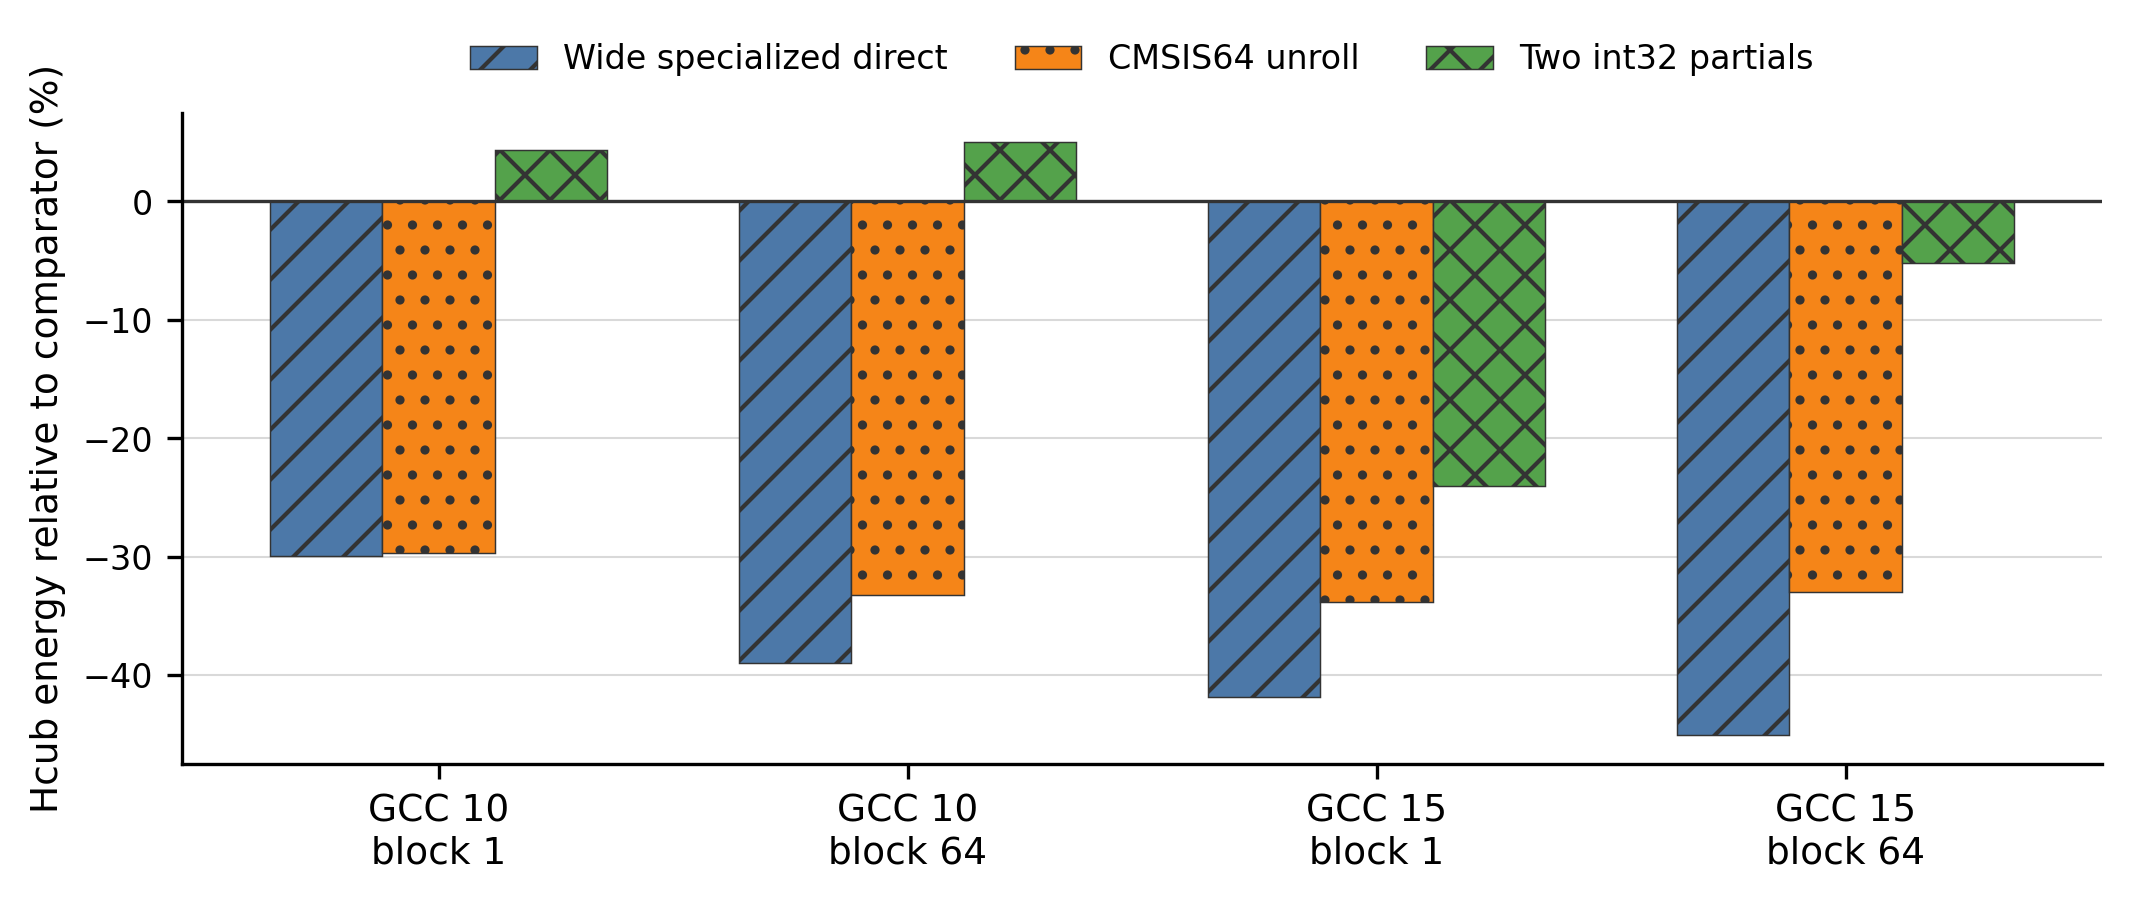
\includegraphics[width=\textwidth]{figures/baseline-robustness.png}
\caption{Hcub relative modeled energy in four fixed configurations, with separately labeled historical and corrected comparator denominators. Crossing zero after direct correction changes the implementation decision.}\label{fig:figures-baseline-robustness.png}
\end{figure*}

The arithmetic correction therefore changes more than the size of an
attractive speedup. In GCC10/block64 the same partial-direct source
organization reduces modeled energy from 990.40 to 575.81 nJ/output
relative to wide direct, and RAM writes over the stream fall from 25,497
to 1,848. It then beats Hcub even though Hcub executes fewer
instructions and native multiplications. Table 4 shows the corresponding
event tradeoff. Under this model, arithmetic reductions do not
compensate for the additional RAM traffic. The observation concerns
these complete binaries; it does not equate one source addition or graph
node with one target instruction.

\begin{table*}[!t]
\centering\footnotesize
\caption{Fewer instructions and MULs coexist with higher complete modeled cost.}\label{tab:4}
\begin{tabularx}{\textwidth}{@{}>{\raggedright\arraybackslash}X>{\raggedright\arraybackslash}X>{\raggedright\arraybackslash}X@{}}
\toprule
GCC10/block64 metric & Partial direct & Hcub \\
\midrule
Instructions & 129,481 & 116,139 \\
Native MUL & 2,827 & 257 \\
RAM reads & 13,695 & 24,689 \\
RAM writes & 1,848 & 20,083 \\
Estimated cycles/output & 583.31 & 636.40 \\
Modeled nJ/output & 575.81 & 604.62 \\
\bottomrule
\end{tabularx}
\end{table*}

The separate incremental-sharing comparison is also mixed. Hcub costs
more modeled energy than ordinary transposition at GCC10/block1 and less
at the other three cells. For GCC15/block64 its 32.94\% saving against
CMSIS becomes 6.69\% against ordinary transposition and 5.23\% against
partial direct. Each percentage is valid for its named question. Only
the ordinary-transposed comparison holds the suffix-state equations
fixed while changing product sharing; none justifies assigning the
entire library gap to Hcub.

Compiler choice changes the feasible alternatives again. With GCC15
fixed, Hcub is 24.06\% and 5.23\% below partial direct. If either tested
compiler may be chosen separately for each form, the best Hcub is GCC15
and the best partial direct is GCC10. The corresponding Hcub modeled
savings are 3.97\% for block1 and 2.30\% for block64. These are minima
over the tested builds, not optimality claims or calibrated physical
improvements. The much smaller margins show why a report must say
whether compiler selection is fixed or part of the implementation
decision.

\section{A partial generated-code explanation}\label{a-partial-generated-code-explanation}

The corrected direct implementation itself is compiler-sensitive. In
block1, GCC15 uses 242,490 instructions, 43,182 RAM reads and 36,500 RAM
writes; GCC10 uses 198,670, 29,304 and 17,225. Their source,
coefficients, input, output contract and native partial structure agree.
A larger frame alone cannot explain executed traffic: allocating stack
space does not write its contents. We therefore examine actual saved
instructions, control flow and source-value lifetimes for these two
binaries.

\subsection{What differs and what does not}\label{what-differs-and-what-does-not}

Both builds retain two native-width partials, sign-extend their
completed values and combine low/high words with \texttt{ADDS/ADCS}
before the single quantizer. Both execute eleven native MULs per output.
Both save and restore nine ABI words per call and materialize the
partial-to-wide interface with four stores and four reloads. These
shared features rule out extra multiplications, additional preserved
registers or a return to wide per-tap accumulation as explanations of
the RAM delta.

GCC15 preloads a set of history samples and retains a sliding window
through registers and stack slots across possible output iterations. Its
tail rotates these values before checking whether another output is
required. GCC10 loads most history samples near use and carries one
sample forward. For block1, each call has only one output; GCC15 still
pays the sample initialization and rotation costs. The runtime block
argument and separate compilation without LTO leave a general loop in
the emitted function. This observation identifies what executes, not
which compiler transformation selected it.

One representative slot demonstrates the required definition/use/update
chain. Here \texttt{h\_i} denotes the chronological history element at
index \texttt{i} in the current output iteration, rather than a filter
coefficient. GCC15 initializes \texttt{{[}sp,\#40{]}} with sample
\texttt{h\_45}, consumes it in the coefficient-12990 product, and
replaces it with old \texttt{h\_46} for a possible next iteration. The
selected tail excerpt below omits other rotations without changing their
ordering.

\begin{Verbatim}[breaklines,breakanywhere,breaksymbolleft={},breaksymbolright={},fontsize=\scriptsize]
080004d4  ldr r2, [sp, #40]   ; old h_45, previously used in convolution
080004d8  mov ip, r2          ; would become next h_44
080004da  ldr r2, [sp, #52]   ; old h_46
080004de  str r2, [sp, #40]   ; would become next h_45
          ...
08000522  ldr r4, [sp, #32]   ; old h_1
08000524  str r4, [sp, #128]  ; would become next h_0
          ...
0800052c  cmp r4, r3          ; output end-pointer test
0800052e  beq 0x08000532      ; block1 exits after rotations
\end{Verbatim}

The frozen annotation records the slot definition at
\texttt{0x08000052/56} and arithmetic use at \texttt{0x0800016c/6e}.
Other slots also hold sample or loop-control values, and a single offset
can have different identities at different times. These facts warrant
``stack-resident values.'' They do not establish that every access is a
register-allocation spill.

\subsection{From static instructions to executed transfers}\label{from-static-instructions-to-executed-transfers}

Aggregate event logs are not per-PC traces. Counting syntactic SP
accesses would therefore be insufficient. In this fixture, the saved
stream wrapper passes \texttt{b=1} on all 257 calls. Copy-in and the
output loop each execute once per call. The 47-iteration history-copy
body has no direct SP-relative access, and neither does any alternative
inside the quantizer. All quantizer paths join before the common output
tail. SP remains fixed between allocation and deallocation, and the body
has no internal calls. The zero-block path is unreachable; GCC10's store
at \texttt{0x08000406} must consequently be excluded.

These path facts give executed direct-SP loads/stores of 9/9 per call
with GCC10 and 63/84 with GCC15. Across the stream the differences are
exactly 13,878 reads and 19,275 writes, equal to the entire saved
RAM-event increase. Other RAM work reconciles equally: each call reads
48 convolution samples, one input, 47 history-copy samples and nine
restored ABI words, and writes one copied input, one output, 47 retained
samples and nine saved ABI words. The stream wrapper adds six reads and
six writes once. This frequency argument connects assembly to event
totals without pretending to possess a dynamic instruction trace.

\subsection{Attributed cost and residual}\label{attributed-cost-and-residual}

Every extra direct-SP load/store contributes one instruction and one RAM
event. Applying the unchanged additive models gives Table 5. All MUL,
Flash-read, Flash-write and BL deltas are zero. The traffic accounts for
85.0151\% of the total modeled energy increase, with that
GCC15-minus-GCC10 increase as the denominator. The remaining
instructions and branches retain their modeled cost.

\begin{table*}[!t]
\centering\footnotesize
\caption{Accepted partial attribution for two existing direct binaries.}\label{tab:5}
\begin{tabularx}{\textwidth}{@{}>{\raggedright\arraybackslash}X>{\raggedright\arraybackslash}X>{\raggedright\arraybackslash}X>{\raggedright\arraybackslash}X@{}}
\toprule
GCC15 minus GCC10, block1 & Total delta & Extra SP transfers & Residual \\
\midrule
Instructions & 43,820 & 33,153 & 10,667 \\
RAM reads & 13,878 & 13,878 & 0 \\
RAM writes & 19,275 & 19,275 & 0 \\
Taken branches & 131 & 0 & 131 \\
Estimated cycles & 77,235 & 66,306 & 10,929 \\
Modeled CPU energy, nJ & 70,469.699925 & 59,909.909673 & 10,559.790252 \\
\bottomrule
\end{tabularx}
\end{table*}

\begin{figure*}[!t]
\centering
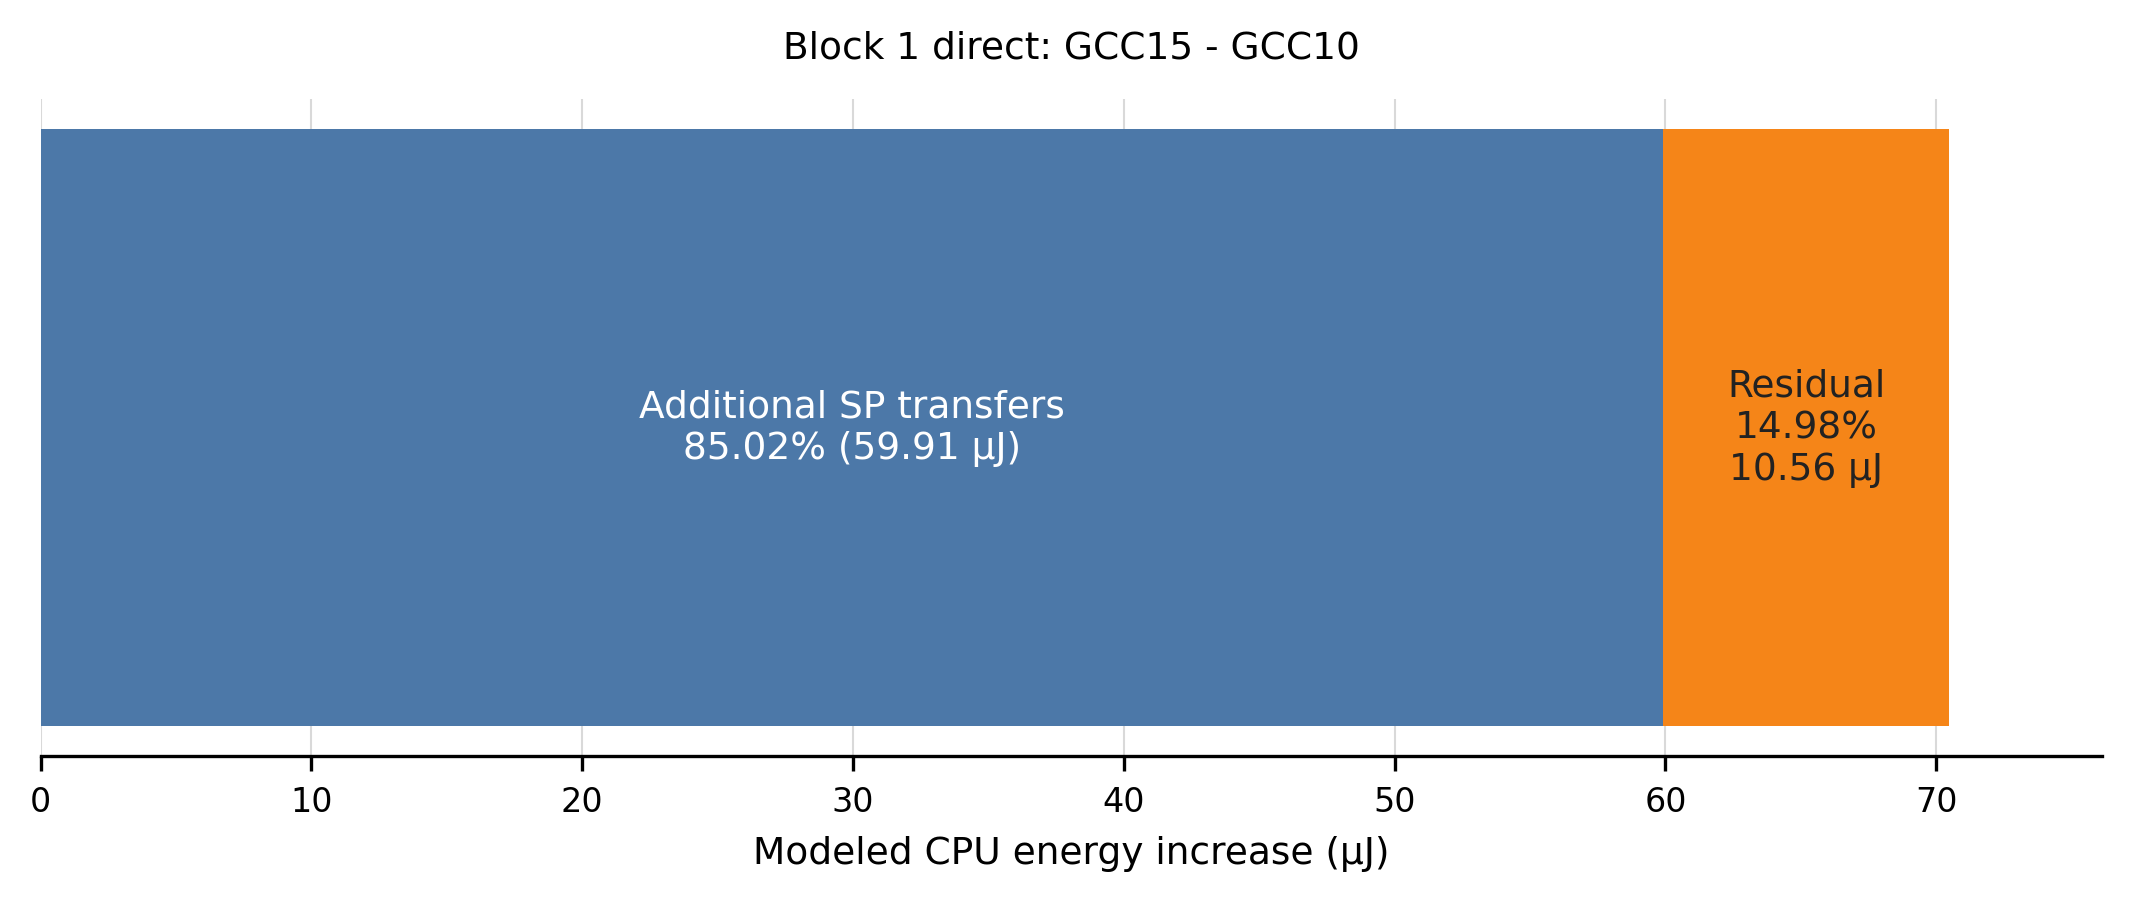
\includegraphics[width=\textwidth]{figures/stack-attribution.png}
\caption{GCC15-minus-GCC10 block1 direct modeled energy: extra direct-SP transfers account for 85.02\% of the increase, with the residual explicitly unassigned.}\label{fig:figures-stack-attribution.png}
\end{figure*}

The two-row accounting passed independent numerical admission, including
29 evidence hashes and reconciliation with the original raw events.
Regeneration reproduced the accounting and hashed analysis files
byte-for-byte. Subsequent manual PC, path and value-flow review accepted
the bounded attribution above. An automated consistency result cannot
certify semantic labels or causation; the manual evidence is essential.
Likewise, the accounting's seven named components contain attributed
subsets, not exhaustive costs of source phases. Events outside those
subsets remain unattributed.

This is an additive cost explanation, not the predicted energy saving
from deleting stack accesses. A different schedule could change many
other events. The responsible compiler pass, reason for stack placement
and remaining instruction/branch difference are unproved. No
counterfactual build or compiler pass trace was collected. The result
also does not explain block64 or the transposed binaries by analogy. Its
scope is the saved pair, sufficient to show why source-level arithmetic
sameness does not imply equal implementation cost in this comparison.

\section{Discussion and threats to validity}\label{discussion-and-threats-to-validity}

\subsection{What the rejected hypothesis establishes}\label{what-the-rejected-hypothesis-establishes}

The central result is a failure of comparator robustness: a prior
four-case advantage becomes a two-case advantage after direct arithmetic
receives certified native-width partials. The rejection is informative
because the old control was plausible for a sum exceeding int32, the
alternative preserves exact semantics, and its outcome depends on
compiler. The range calculation alone cannot predict that split. The
observed event tradeoff and bounded stack-value account supply evidence
beyond the elementary statement that a sum can be partitioned safely.

The strongest objection is that this remains a selected example of
standard engineering rather than a broadly novel optimization method.
That objection limits the contribution appropriately. We do not derive a
general selection rule, invent range-aware FIR generation, optimize the
partition or establish that Hcub's graph objective should be changed.
The useful result is an audited counterexample to treating the earlier
local decision as stable under a stronger control. The positive GCC15
cases are as important as the negative GCC10 cases: reporting only
either pair would misrepresent the assessment.

H\_R's retrospective formulation also limits its epistemic role. Its
rejection organizes already-observed evidence rather than providing an
independently predicted discovery. The exact four-case rule prevents
flexible redefinition of success within the paper, but cannot undo
filter selection or inspection of earlier results. A future
generalization claim would need independently chosen workloads and
equally strong controls throughout; it does not follow from repackaging
this finite case as a statistical sample.

\subsection{Internal validity and interpretation}\label{internal-validity-and-interpretation}

Bit-exact output agreement, retained-state checks, guards, full-domain
bounds and assembly review address different failure modes. None alone
guarantees all the others. Independent decoding reduces reliance on a
shared expected output implementation, while frozen artifact identities
connect reported events to the binaries that were checked. These checks
support the comparison but do not make the stronger direct control
optimal. An alternative grouping, schedule, compiler option or
implementation could change the minimum.

The energy model weights correlate with aggregate execution events.
Event attribution under that model is legitimate arithmetic, but
physical causality requires more evidence. In particular, frame size is
not a traffic count, all stack temporaries are not demonstrated spills,
and a large attributed fraction does not identify a faulty compiler
pass. The residual in Table 5 prevents the partial account from being
mistaken for a complete generated-code explanation. Estimated-cycle
agreement with energy winners supplies another reported metric, not
independent hardware validation.

\subsection{External validity and resource tradeoffs}\label{external-validity-and-resource-tradeoffs}

The all-int16 arithmetic proof has a broader domain than the performance
observations. Costs were observed for one finite saved stream, zero
initial history, a selected nonsymmetric filter, two blocks and two
compiler builds. Startup and call work can matter greatly at block1,
while input-dependent quantizer paths may differ for another stream. The
257 samples and separate edge tests are not independent application
trials. These already-inspected cases cannot establish steady-state or
population-wide FIR behavior.

The Cortex-M0 label also does not identify every physical implementation
choice. Single-cycle MUL, zero wait states and the selected
prefetch/frequency configuration are explicit model assumptions. No
board current, peripheral energy, end-to-end latency or physical
uncertainty calibration was measured. Small compiler-selectable modeled
margins therefore cannot support a physical winner claim. Transferring
the results to another core, memory configuration, compiler flags or
library version would require its own evidence.

Energy is only one decision dimension. Direct state allocation is 98
bytes at block1 and 224 at block64; transposed allocation is 192 in both
cases. Partial direct has smaller reported frames than the transposed
controls here, while code-size ordering depends on the chosen
comparison. The reported frame is only \texttt{probe\_process};
selected-symbol bytes exclude fixture code and may omit other helpers.
Neither metric establishes peak SRAM or total executable size. A
deployment with a strict memory budget must examine those quantities
explicitly rather than reading the energy winner as a complete system
choice.

\section{Conclusion}\label{conclusion}

Demand-Hcub's earlier modeled advantage over both wide specialized
direct and unrolled CMSIS does not survive a stronger arithmetic-fair
direct control in all four fixed configurations. H\_R is rejected:
partial direct wins both GCC10 cases, while Hcub wins both GCC15 cases.
The saved block1 direct binaries further support a partial
generated-code account: extra executed direct-SP transfers explain all
added RAM traffic and 85.02\% of the GCC15 modeled energy increase, with
a retained residual and unresolved compiler cause. This case shows why
an exact arithmetic contract, a strong comparator and complete execution
costs are necessary to interpret a sharing result. Its conclusion is
bounded to the frozen filter, stream, builds and models; it introduces
no new FIR algorithm and makes no physical energy claim.

\begin{thebibliography}{99}

\bibitem{1} L. De Coster, M. Adé, R. Lauwereins, and J. A. Peperstraete, ``Code
Generation for Compiled Bit-True Simulation of DSP Applications,'' in
\emph{Proceedings of the 11th International Symposium on System
Synthesis}, 1998, pp.~9--14.
\href{https://cecs.uci.edu/~papers/compendium94-03/papers/1998/isss98/pdffiles/1_2.pdf}{Primary
manuscript}.

\bibitem{2} A. Gačić, M. Püschel, and J. M. F. Moura, ``Fast Automatic Software
Implementations of FIR Filters,'' in \emph{Proceedings of IEEE ICASSP},
vol.~II, 2003, pp.~541--544, doi: 10.1109/ICASSP.2003.1202423.
\href{https://users.ece.cmu.edu/~moura/papers/icassp03-gacic-pueschel-ieeexplore.pdf}{Author
manuscript}.

\bibitem{3} P. D'Alberto, M. Püschel, and F. Franchetti, ``Performance/Energy
Optimization of DSP Transforms on the XScale Processor,'' in
\emph{HiPEAC 2007}, LNCS 4367, 2007, pp.~201--214.
\href{https://users.ece.cmu.edu/~franzf/papers/hipeac07.pdf}{Author
manuscript}.

\bibitem{4} Y. Voronenko and M. Püschel, ``Multiplierless Multiple Constant
Multiplication,'' \emph{ACM Transactions on Algorithms}, vol.~3, no. 2,
Art. 11, May 2007, doi: 10.1145/1240233.1240234.
\href{https://spiral.ece.cmu.edu/pubs/synth.pdf}{Author manuscript}.

\bibitem{5} K. Nikov, K. Georgiou, Z. Chamski, K. Eder, and J. Nunez-Yanez,
``Accurate Energy Modelling on the Cortex-M0 Processor for Profiling and
Static Analysis,'' in \emph{2022 29th IEEE International Conference on
Electronics, Circuits and Systems (ICECS)}, 2022, pp.~1--4, doi:
10.1109/ICECS202256217.2022.9971086. Accessible version:
arXiv:2301.12806v1, 2023.
\href{https://arxiv.org/html/2301.12806v1}{Primary paper}.

\end{thebibliography}

\appendices

\section{Resource diagnostics for every principal row}\label{appendix-a.-resource-diagnostics-for-every-principal-row}

Tables 6 and 7 use the artifact variant identifiers from Table 1. Cycles
are Arm-table estimates per requested output. Code means selected kernel
and coefficient symbols, excluding fixture code and potentially other
helpers. Frame means the compiler's static \texttt{probe\_process}
frame; callee frames are separately preserved in the admitted
verification JSON. State is the allocated state object, including its
block capacity. These are not total image size, peak live stack or SRAM
high-water measurements.

\begin{table*}[!t]
\centering\footnotesize
\caption{GCC10 resource diagnostics for every principal row.}\label{tab:6}
\begin{tabularx}{\textwidth}{@{}>{\raggedright\arraybackslash}X>{\raggedright\arraybackslash}X>{\raggedright\arraybackslash}X>{\raggedright\arraybackslash}X>{\raggedright\arraybackslash}X>{\raggedright\arraybackslash}X@{}}
\toprule
Compiler/block & Variant & Cycles/output & Code bytes & State bytes & Frame bytes \\
\midrule
GCC10/1 & CMSIS & 1585.11 & 1494 & 112 & 8 \\
GCC10/1 & Wide direct & 1606.11 & 1736 & 98 & 440 \\
GCC10/1 & Partial direct & 1065.11 & 1036 & 98 & 72 \\
GCC10/1 & Ordinary transposed & 1106.11 & 1540 & 192 & 272 \\
GCC10/1 & Hcub & 1150.11 & 1504 & 192 & 344 \\
GCC10/64 & CMSIS & 924.32 & 1494 & 236 & 8 \\
GCC10/64 & Wide direct & 1029.33 & 1720 & 224 & 440 \\
GCC10/64 & Partial direct & 583.31 & 1196 & 224 & 72 \\
GCC10/64 & Ordinary transposed & 630.64 & 1540 & 192 & 272 \\
GCC10/64 & Hcub & 636.40 & 1504 & 192 & 344 \\
\bottomrule
\end{tabularx}
\end{table*}

\begin{table*}[!t]
\centering\footnotesize
\caption{GCC15 resource diagnostics for every principal row.}\label{tab:7}
\begin{tabularx}{\textwidth}{@{}>{\raggedright\arraybackslash}X>{\raggedright\arraybackslash}X>{\raggedright\arraybackslash}X>{\raggedright\arraybackslash}X>{\raggedright\arraybackslash}X>{\raggedright\arraybackslash}X@{}}
\toprule
Compiler/block & Variant & Cycles/output & Code bytes & State bytes & Frame bytes \\
\midrule
GCC15/1 & CMSIS & 1550.11 & 1450 & 112 & 8 \\
GCC15/1 & Wide direct & 1798.11 & 1872 & 98 & 608 \\
GCC15/1 & Partial direct & 1365.63 & 1372 & 98 & 240 \\
GCC15/1 & Ordinary transposed & 1100.11 & 1532 & 192 & 272 \\
GCC15/1 & Hcub & 1062.11 & 1352 & 192 & 344 \\
GCC15/64 & CMSIS & 851.98 & 1450 & 236 & 8 \\
GCC15/64 & Wide direct & 1074.65 & 1884 & 224 & 608 \\
GCC15/64 & Partial direct & 612.39 & 1312 & 224 & 232 \\
GCC15/64 & Ordinary transposed & 627.57 & 1532 & 192 & 272 \\
GCC15/64 & Hcub & 593.49 & 1352 & 192 & 344 \\
\bottomrule
\end{tabularx}
\end{table*}

\section{Frozen identities and evidence locations}\label{appendix-b.-frozen-identities-and-evidence-locations}

The coefficient and timed-input identities recorded by the
partial-direct experiment are:

\begin{Verbatim}[breaklines,breakanywhere,breaksymbolleft={},breaksymbolright={},fontsize=\scriptsize]
coefficient SHA256:
\end{Verbatim}
\noindent\texttt{\scriptsize\seqsplit{63796e3e365dbdee70192acf68f16f403802d961df48ae814ffb23cca411fb70}}\par
\begin{Verbatim}[breaklines,breakanywhere,breaksymbolleft={},breaksymbolright={},fontsize=\scriptsize]
timed-input SHA256:
\end{Verbatim}
\noindent\texttt{\scriptsize\seqsplit{d952c2754c9ae922243966a9c2533a848b345aa2d2d6cb5b4e68d9df1615f310}}\par
\begin{Verbatim}[breaklines,breakanywhere,breaksymbolleft={},breaksymbolright={},fontsize=\scriptsize]
partial-direct kernel.c SHA256:
\end{Verbatim}
\noindent\texttt{\scriptsize\seqsplit{5832b52eaf1d5eb76e8087d47307feeccf74809cc0f22b288d111505851501cd}}\par

The four partial-direct target binary identities are:

\begin{Verbatim}[breaklines,breakanywhere,breaksymbolleft={},breaksymbolright={},fontsize=\scriptsize]
GCC10/block1
\end{Verbatim}
\noindent\texttt{\scriptsize\seqsplit{07fd7023d12ead52fee14a266c647627d664f37c18c234a0b41e2f226f143a6a}}\par
\begin{Verbatim}[breaklines,breakanywhere,breaksymbolleft={},breaksymbolright={},fontsize=\scriptsize]
GCC10/block64
\end{Verbatim}
\noindent\texttt{\scriptsize\seqsplit{fb08c19043261b1db7644a8ca4f0749f46b893e51a4d685e2a5cf339fbe23f11}}\par
\begin{Verbatim}[breaklines,breakanywhere,breaksymbolleft={},breaksymbolright={},fontsize=\scriptsize]
GCC15/block1
\end{Verbatim}
\noindent\texttt{\scriptsize\seqsplit{114041b0f03a20c34a9c8a37b147116dff9f74c3c321bd2af4d7709d710e3470}}\par
\begin{Verbatim}[breaklines,breakanywhere,breaksymbolleft={},breaksymbolright={},fontsize=\scriptsize]
GCC15/block64
\end{Verbatim}
\noindent\texttt{\scriptsize\seqsplit{140f1e446715a79b1384f1b46a274c8ac03bb097879b959ad4c7a743a7418638}}\par

The source manifest delivered beside this paper identifies the six
frozen JSON inputs by path and SHA256; generated results identify all
selected rows and binaries. The
\href{../fir-sharing-probe/PROTOCOL.md}{original protocol},
\href{../../docs/superpowers/plans/2026-10-20-fir-baseline-check.md}{fixed
control plan},
\href{../fir-sharing-probe/independent-check/comparison.md}{independent
comparison},
\href{../fir-sharing-probe/independent-check/join-review.md}{manual
join}, and
\href{../fir-sharing-probe/explanation-check/final-decision.md}{final
explanation decision} preserve the evidence sequence. The
\href{../fir-sharing-probe/compiler-explanation/assembly-notes.md}{assembly
annotation} contains the full definition/use/rotation account and
excluded paths. Frozen automated status strings still mark manual review
pending; the subsequent manual records supply acceptance rather than
silently rewriting those strings.

The historical 12/24 bank statistic belongs to its original candidate
set. There is no revised bank-wide result using equally narrowed direct
controls, and none is inferred by this manuscript.

\section{Reproduction levels}\label{appendix-c.-reproduction-levels}

The paper can be regenerated from saved results without compiling a
target or executing the simulator. From the repository root, run:

\begin{Verbatim}[breaklines,breakanywhere,breaksymbolleft={},breaksymbolright={},fontsize=\scriptsize]
python3 research/fir-paper/build_results.py --output-dir research/fir-paper
\end{Verbatim}

This writes the auditable selected results, derived tables and source
manifest. The \href{README.md}{paper README} documents the test, figure
and IEEE conference PDF build commands and the exact output artifacts.
The tool freezes source bytes, cross-checks selected totals and computes
hypothesis outcomes; it does not replace the historical raw-evidence
check or manual semantic review.

For the admitted partial-direct evidence, restore the versioned archive
before running the independent checker if its raw build directories are
absent:

\begin{Verbatim}[breaklines,breakanywhere,breaksymbolleft={},breaksymbolright={},fontsize=\scriptsize]
sha256sum -c \
  research/fir-sharing-probe/independent-check/partial-direct-target-evidence.sha256
tar -xzf \
  research/fir-sharing-probe/independent-check/partial-direct-target-evidence.tar.gz \
  -C research/fir-sharing-probe/partial-direct
python3 research/fir-sharing-probe/independent-check/check.py \
  --peer-results research/fir-sharing-probe/partial-direct/results.json
\end{Verbatim}

The
\href{../fir-sharing-probe/independent-check/README.md}{independent-check
README} documents historical raw-artifact requirements; those ignored
build artifacts are not guaranteed by an ordinary checkout. Full target
reproduction additionally requires the pinned toolchains and simulator
described in the \href{../fir-baseline/README.md}{baseline README}. The
\href{../fir-sharing-probe/explanation-check/README.md}{explanation-check
README} provides independent accounting verification. Distinguish table
regeneration, saved-artifact admission and a new target execution when
reporting which level was actually performed.
\end{document}
